\subsection{Problema a resolver}


\subsection{Resolución coloquial}


\subsection{Demostración de correctitud}

Primero veamos el invariante de nuesta solucion:
\begin{itemize}
\item Sea S una solucion, cumple que el i-esimo curso tiene la fecha de finalizacion mas proxima posible\footnote{Con "posible" nos referimos a que no se solapa con ningun curso que tenga menor fecha de finalizacion.} al anterior, es decir, al (i-1)-esimo curso. Estando siempre el curso que primero finaliza como solucion.
\end{itemize}

Sea C un conjunto de cursos tal que:
\begin{itemize}
\item Ningun curso se solapa, la solucion es C. Esto es trivial, ya que mas cursos de los que hay no pueden  haber.
\item Existen dos cursos que se solapan. Sea $i$ y $j$ dichos cursos. Sin perder generalidad supongamos que la fecha de terminacion de $j$ es mayor o igual que la de $i$. Quiero ver que, si S es la solucion que contiene a $i$ y S' es la solucion que contiene a $j$ $\Rightarrow$ $|$S'$|$ $\leq$ $|$S$|$. 
  Esto se cumple porque S' contiene a $j$ que termina luego que $i$, por lo que por lo menos todos los cursos de S' desde el $j$ estan contenidos en S y, ademas, si  $j$ comienza antes que $i$ se que la cantidad de cursos de S' antes de $j$ estan antes de $i$ en S 

\begin{figure}[H] %[h] Aqui [b] para button [t] para top
\begin{center}
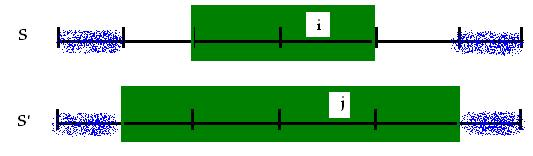
\includegraphics[width=322pt]{../imgs/demo21.jpg}
\end{center}
\end{figure}

ò si $j$ empieza luego de $i$ yo se que no termina ningun otro curso entre el comienzo de $i$ y $j$, porque de terminar ubiese elejido ese en S  (ya que elijo siempre el que termina antes), 

\begin{figure}[H] %[h] Aqui [b] para button [t] para top
\begin{center}
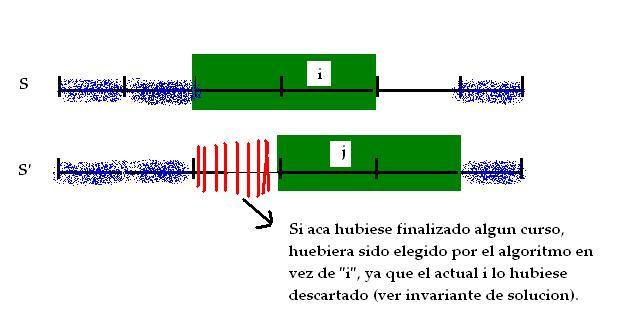
\includegraphics[width=322pt]{../imgs/demo22.jpg}
\end{center}
\end{figure}

\end{itemize}

por lo tanto, $|$S'$|$ $\leq$ $|$S$|$. 


\subsection{Complejidad del algoritmo}

Sea $n$ la cantidad de cursos . La complejidad de nuestro algoritmo es $O(n.log n)$, antes de ver el porque de esto tengamos en cuenta algunos aspectos:
\begin{enumerate}
\item La complejidad del algoritmo \textbf{Sort} es $O(n.log n)$. Referencia en: http://en.cppreference.com/w/cpp/algorithm/sort donde dice $"$O(N.log(N)), where N = std::distance(first, last) applications of cmp $"$ y nuestra funcion de comparacion es constante ya que solo compara dos tuplas.
\item La complejidad del \textbf{constructor} que utilizamos sobre la estructura \textbf{vector} es $O(1)$. Referencia en:http://en.cppreference.com/w/cpp/container/vector/vector .
\item La complejidad del algoritmo \textbf{push$\_$back} sobre la estructura \textbf{vector} es O(1) amortizado. Referencia en: http://en.cppreference.com/w/cpp/container/vector/push$\_$back. 
\item La complejidad del algoritmo \textbf{size} sobre la estructura \textbf{vector} es O(1). Referencia en: http://en.cppreference.com/w/cpp/container/vector/size.
\item La complejidad de la funcion \textbf{filtrarSolapamientos} es $O(n)$ ya que va recorriendo los cursos, comparando y agregando elementos segun corresponda (comparar es constante al igual que agregar y recorrer lineal), en otras palabras, se encuentra un \textbf{if} (complejidad constante) y un \textbf{push$\_$back} (complejidad constante) dentro de un \textbf{for} (complejidad lineal). 
\end{enumerate}
Teniendo en cuenta lo anterior el siguiente grafico muestra el codigo y al costado la complejidad de cada operacion.

\begin{figure}[H] %[h] Aqui [b] para button [t] para top
\begin{center}
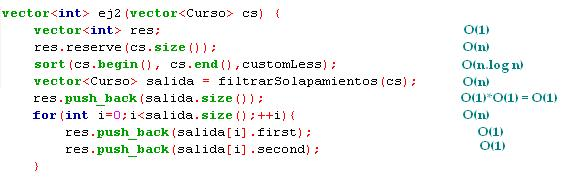
\includegraphics[]{../imgs/comple2.jpg}
\end{center}
\end{figure}

Finalmente, la complejidad es: $O(1)+O(n)+O(n.log n)+O(n)+O(1)+O(n)*O(1)*O(1)$ = \textbf{O(n.log n)}

\subsection{Código fuente}



\subsection{Instancias posibles}



\subsection{Testing}
